\documentclass[a4paper]{article}
\usepackage{amsthm}
\usepackage{amssymb}
\usepackage{amsbsy}
\usepackage{amsmath}
\usepackage[
  margin=1.5cm,
  includefoot,
  footskip=30pt,
]{geometry}
\usepackage{layout}
\usepackage{graphicx}
\title{Probabilistic Graphical Models : Homework 3}
\author{Raphael Avalos\\raphael@avalos.fr}
\graphicspath{ {./plots/} }
\begin{document}
\maketitle
\section*{Equations}
Writing the complete log likelihood and applying the method for EM we get the following equations.
\begin{align*}
\pi &= p(q_0 \mid u)\\
A_{i,j} &= \frac{\sum_t p(q_{t+1} = i, q_t=j \mid u)}{\sum_{i,t} p(q_{t+1} = i, q_t=j \mid u)} \\
\mu_k &= \frac{\sum_t p(q_t = k \mid u) u_t}{\sum_t p(q_t = k \mid u)}\\
\Sigma_k &= \frac{\sum_t p(q_t = k \mid u) (u_t - \mu_k)(u_t - \mu_k)^T}{\sum_t p(q_t = k \mid u)}\\
\end{align*} 



\section*{Results}
\begin{tabular}{|c|c|c|c|}
\hline 
Log Likelihood & Iso & General & HMM\\ 
\hline 
Train & $-2682$ & $-2345$ & $-1899$\\ 
\hline 
Test  & $-2733$ & $-2426$ & $-1959$\\
\hline
\end{tabular}
\\\\


\begin{figure}[h]

\begin{minipage}{0,95\textwidth}
\caption{HMM vs GMM}
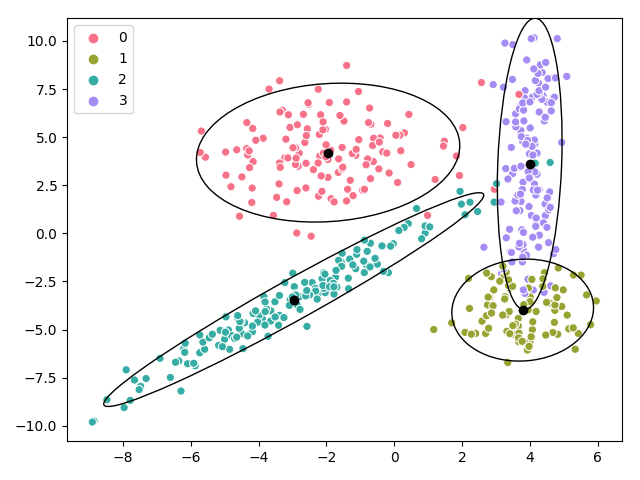
\includegraphics[scale=.40]{train.png}
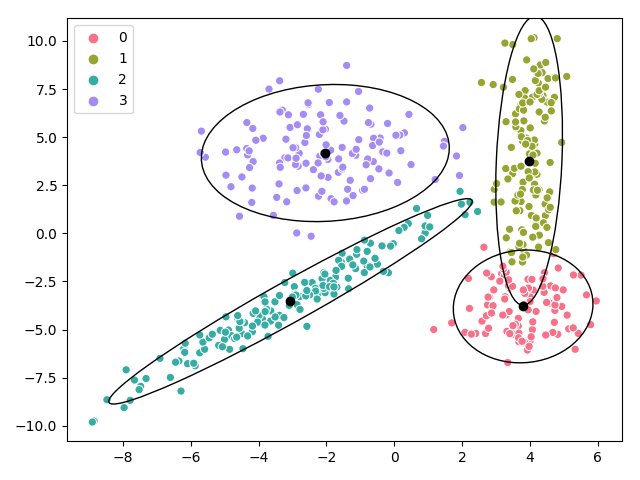
\includegraphics[scale=.40]{em_general.png}
\end{minipage}
\end{figure}

HMM seems to take into account the fact that the categories overlapse compared to GMM. The log likelihood increase significantly so we have more confidence in the HMM model.

\end{document}
